% !TeX root = ../main.tex
% Add the above to each chapter to make compiling the PDF easier in some editors.

\chapter{Background and Related Work}\label{chapter:background}

We explain two research fields that create the bedrock of this thesis, namely, fake news detection and explainable artificial intelligence.
Both areas provide the foundation of tools that were used in this work. The first provides the mechanisms and approaches to detect fake news,
and the second offers a suite of techniques to interpret these mechanisms and approaches.\\
Initially, in \ref{sec:fakeNewsDetection}, we discuss societal challenges, the characteristics, and the history of fake news. Then we talk about the detection methods that were developed over the years. After showing the challenges of creating FND models, we conclude the first section with SOTA FND models.\\
After fake news detection, in \ref{sec:explainableArtificialIntelligence}, we first examine when XAI is necessary and its importance. Then, we define the suite of explainable artificial intelligence and the goals of XAI, and finally, we determine the suite that aims to satisfy these goals.\\
\section{Fake News Detection}
\label{sec:fakeNewsDetection}
In the past decade, social media has become a place where anyone can share information. Although fast, free, and easy to access, obtaining
real news from social media can be difficult, and one should do so at their own risk and always check the
facts~\parencite{SocialMediaAndFakeNewsIn2016Election_Allcott,TheScienceOfFakeNews_Lazer}. But the news stream never ends; thus, the need to verify the credibility of news using automated systems arises. To address this necessity, the number of studies involving \emph{Fake News} or \emph{Fake News Detection} has dramatically increased in the last decade (Fig. \ref{fig:FN_vs_FND_Publications}).
\begin{figure}
    \centering
    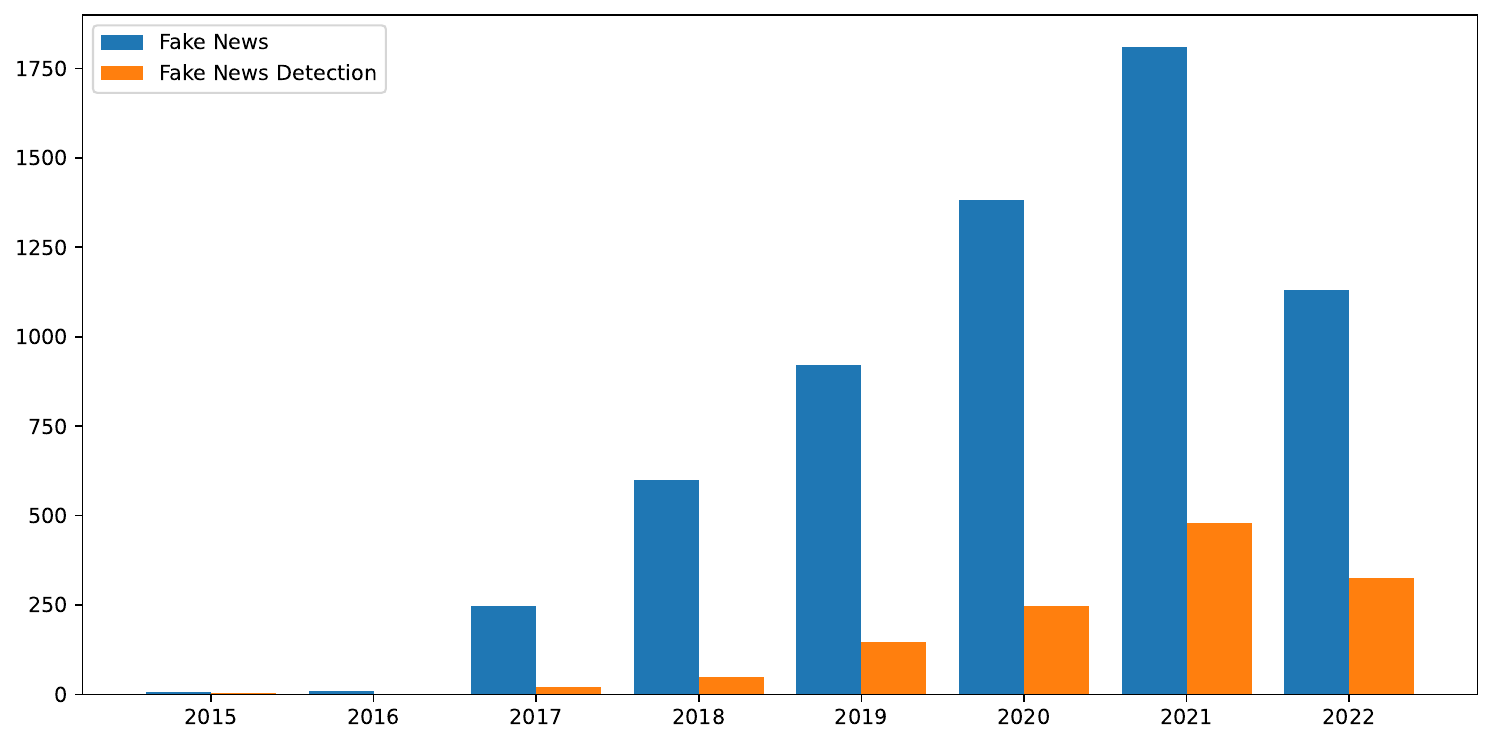
\includegraphics[scale=0.5]{FN_vs_FND_Publications}
    \caption[Fake News and Fake News Detection Publications by Year]{Total number of publications that include (1) \emph{Fake News} (blue) and (2) \emph{Fake News Detection} (orange) publications by year. Source: Scopus; Search Arguments: (1) TITLE-ABS-KEY("fake news*") PUBYEAR AFT 2014 (2) TITLE-ABS-KEY("fake news detection")}\label{fig:FN_vs_FND_Publications}
\end{figure}\\
In \ref{subsec:fakeNewsDetection_fakeNews}, we briefly present the history of fake news and look at studies that display the impact of fake news on society. In this section, we also define the terms fake news, disinformation, and misinformation. \\
In \ref{subsec:fakeNewsDetection_FoundationsOfFakeNews}, we make an excursion into social sciences and human psychology, delivering insights into why humans fall for or tend to believe fake news. Furthermore, we draw some insights from the socio-technical foundations of fake news.\\
We then list the available datasets used in FND and talk about their advantages and disadvantages in \ref{subsec:fakeNewsDetection_Evolution}. Finally, in \ref{subsec:fakeNewsDetection_Evolution}, we first talk about the evolution of detection algorithms, then we classify FND algorithms with respect to their input data type and what they focus on that data.\\
\subsection{Fake News}
\label{subsec:fakeNewsDetection_fakeNews}
Throughout history, various forms of widespread fake news have been recorded. For instance, in the thirteenth century BC, Rameses the Great decorated his temples with paintings that tell stories of victory in the Battle of Kadesh. However, the treaty between the two sides reveals
that the outcome of the battle was a stalemate~\parencite{HistorysGreatestLies_Weir}. Just after the printing press was invented in 1439,
the circulation of fake news began. One of history's most famous examples of fake news is the
“Great Moon Hoax”~\parencite{TheGreatMoonHoax_Foster}. In 1835, The Sun newspaper of New York published articles about a real-life astronomer and a made-up colleague who had observed life on the moon. It turns out that these fictionalized articles brought them new customersand almost no backlash after the newspaper admitted that the articles mentioned earlier
were a hoax\footnote{https://www.politico.com/magazine/story/2016/12/fake-news-history-long-violent-214535/}.\\
In order to highlight the difference, using the definitions from~\parencite{ThePsycologyOfFakeNews_Pennycook}, we formally define the terms disinformation and misinformation as follows,
\begin{definition}[\emph{Disinformation}]
    Information that is false or inaccurate and was created with a deliberate intention to mislead people.
\end{definition}
\begin{definition}[\emph{Misinformation}]
    Information that is false, inaccurate, or misleading. Unlike disinformation, misinformation does not necessarily need to be created deliberately
    to mislead.
\end{definition}
There is no fixed definition for fake news. Thus, we elaborate on the definitions of fake news. A limited definition is news articles that are intentionally or verifiably false~\parencite{SocialMediaAndFakeNewsIn2016Election_Allcott}. This definition stresses authenticity and intent. The inclusion of false information that can be confirmed refers to authenticity. On the other hand, intent refers to the deceitful intention to delude news consumers~\parencite{FakeNewsDetectionOnSocialMediaADataMiningPerspective_Shu}. This definition is widely used in other studies~\parencite{AutomaticDeceptionDetection_Conroy, TheFakeNewsSpreadingPlague_Mustafaraj, FakeNewsDetectionOnSocialMediaADataMiningPerspective_Shu}.
Furthermore, recent social sciences studies~\parencite{TheScienceOfFakeNews_Lazer, ThePsycologyOfFakeNews_Pennycook} define fake news as fabricated information that mimics news media content in form but not in organizational process or intent. Similarly, this definition covers authenticity and intent; additionally, it includes the organizational process. More general definitions for fake news consider satire news as fake news due to the inclusion of false information even though satire news aim to entertain and inherently reveals its deception to the consumer~\parencite{WhenFakeNewsBecomesReal_Balmas, TheImpactOfRealNewsAboutFakeNews_Brewer, NewsVerificationByExploitingConflictingSocialViewpoints_Jin, FakeNewsOrTruthUsingSatiricalCues_Rubin}. Further definitions include hoaxes, satires, and obvious
fabrications~\parencite{DeceptionDetectionForFakeNews3TypesOfFakeNews_Rubin}
In this thesis, we are not interested in the organizational process and do not consider conspiracy theories~\parencite{ConspiracyTheories_Sunstein}, superstitions~\parencite{Superstition_Lindeman}, rumors~\parencite{RumorsAndHealthCareReform_Berinsky}, misinformation, satire, or hoaxes. Therefore, we use the limited definition from~\parencite{SocialMediaAndFakeNewsIn2016Election_Allcott} and formally introduce it as follows:
\begin{definition}[\emph{Fake News}]
    News articles that are intentionally or verifiably false.
\end{definition}
Fake news can lead to disastrous situations, such as crashes in stock markets, resulting in millions of dollars. For example, Dow Jones
industrial average went down like a bullet (see Fig. \ref{fig:MarketReactionToFakeTweet}) after a tweet about an explosion injuring President Obama
went out due to a hack~\parencite{MarketQuaversAfterFakeAPTweet_ElBoghdady}.
\begin{figure}
    \centering
    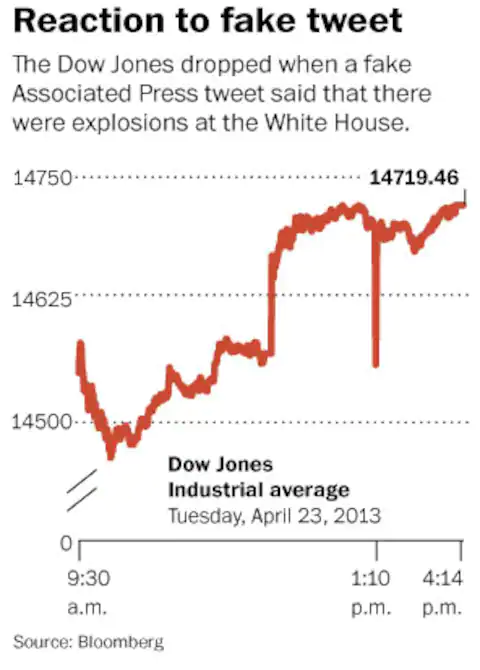
\includegraphics[scale=0.2]{MarketReactionToFakeTweet}
    \caption[Market Reaction to Fake Tweet]{The market's reaction to the fake tweet. The sharp decline caused by a single tweet. Image obtained from~\parencite{MarketQuaversAfterFakeAPTweet_ElBoghdady}}\label{fig:MarketReactionToFakeTweet}
\end{figure}\\
The detrimental impacts of fake news further extend to societal issues.
When fake news rose to prominence with the 2016 U.S. Presidential Election~\parencite{USPresidentialElection2016}, a man, convinced by what he
read on social media about a pizzeria trafficking humans, went on a shooting spree in that pizzeria. Later named
Pizzagate~\parencite{Pizzagate_Fisher}, this incident illustrates the deadly impact of fake news. In fact, fake news can even affect presidential elections~\parencite{SocialMediaAndFakeNewsIn2016Election_Allcott, TrumpWonBecauseOfFacebook_Read}.\\
Recent history exhibits that some fake news spreads like wildfires through social media. Evidence shows that the most popular fake news stories
were more widely shared than the most popular mainstream news stories~\parencite{Buzzfeed_FakeNewsOutperformRealNews_Silverman}.\\
Digital News Report 2022~\parencite{ReutersInstituteDigitalNewsReport} reports in its key findings that trust in the news is 42\% globally,
the highest (69\%) in Finland, and the lowest (26\%) in the U.S.A. Additionally, the same study shows that in early 2022, in the week of the
survey, between 45\% and 55\% of the surveyed social media consumers worldwide witnessed false or misleading information about COVID-19. The
same study also reports the appearance of fake news in politics was between 34\% and 51\%, and between 9\% and 48\% for fake news about
celebrities, global warming, and immigration~\parencite{StatistaUsageOfSocialMedia_Watson}.
\begin{figure}
    \centering
    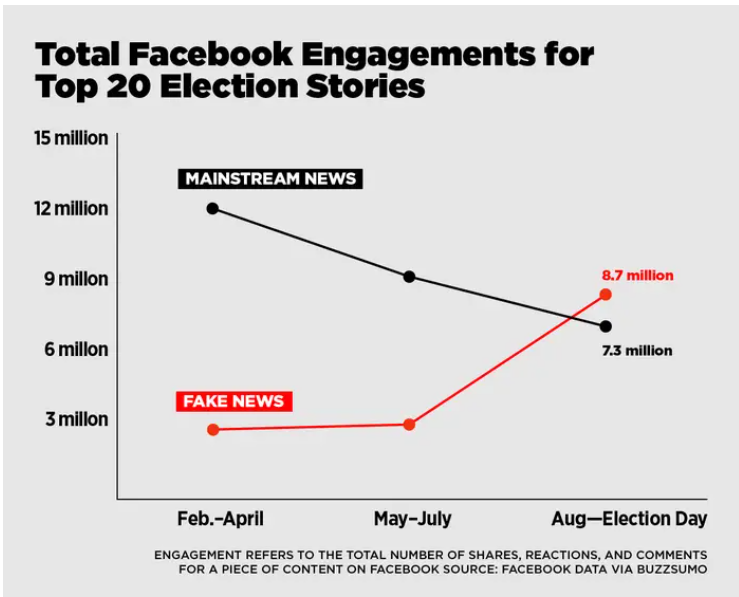
\includegraphics[scale=0.4]{TotalFacebookEngagementsForTop20ElectionStories}
    \caption[Total Facebook Engagements for Top 20 Election Stories]{The rising engagement for fake news stories observed after May-July, just before Presidential Elections. Image obtained from~\parencite{Buzzfeed_FakeNewsOutperformRealNews_Silverman}}\label{fig:TotalFacebookEngagementsForTop20ElectionStories}
\end{figure}
\subsection{Foundations of Fake News}
\label{subsec:fakeNewsDetection_FoundationsOfFakeNews}
The environment for fake news has been the traditional news media for a long time. First started with newsprint, then continued with radio
and television, and now with social media and the web, the dissemination of fake news reached its peak. Next, we discuss the psychological
and social foundations of fake news to stress the importance of human psychology, especially when accepting fake news as genuine and sharing
it with others. Then we focus on the technical foundations where we discuss how social media and technologiy have accelerated the diffusion of
fake news.\\

\textbf{Psychological Foundations.}  Understanding the difference between real and fake news is not an easy task for a human. Two psychological theories, namely, \emph{naive realism} and \emph{confirmation bias}, examine why humans fall for fake news. The first refers to a person's disposition to believe that their point of view is the mere accurate one, while people who believe otherwise are uninformed or biased~\parencite{NaiveRealism_Reed}. The second, often called selective exposure, is the proclivity to prefer information that confirms existing views~\parencite{ConfirmationBias_Nickerson}.\\
Another reason for human fallacy in fake news is that once a misperception is formed, it becomes difficult to correct. In fact, it turns out that correcting people leads them to believe false information more, especially when given factual information that refutes their beliefs~\parencite{WhenCorrectionsFail_Nyhan}.\\

\textbf{Social Foundations.}  The prospect theory explains the human decision-making process as a mechanism based on maximizing relative gains and minimizing losses with respect to the current state~\parencite{ProspectTheory_Kahneman, AdvancesInProspectTheory_Kahneman}. This inherent inclination to get the highest reward also applies to social cases in which a person will seek social networks that provide them with social acceptance. Consequently,  people with different views tend to form separate groups, which makes them feel safer, leading to the consumption
and dissemination of information that agrees with their opinions. These behaviors are explained by social identity
theory~\parencite{SocialIdentityTheory_Ashforth} and normative social influence~\parencite{NormativeSocialInfluence_Asch}.
Two psychological factors play a crucial role here~\parencite{TheRussianFirehoseOfFalsehood_Paul}. The first, social credibility, is explained
by a person’s tendency to recognize a source as credible when that source is deemed credible by other people. The second, called the frequency heuristic, is the acceptance of a news piece by repetitively being exposed to it. Collectively, these psychological phenomena are closely related to the well-known filter bubble~\parencite{TheFilterBubble_Pariser}, also called echo chamber, which is the formation of homogenous bubbles in which the users are people of similar ideologies and share similar ideas. Being isolated from different views, these users usually are inclined to have highly polarized opinions~\parencite{EchoChambers_Sunstein}. As a result, the main reason for misinformation dispersal turned out to be the echo
chambers~\parencite{TheSpreadingOfMisinformationOnline_DelVicario}.\\

\textbf{Technical Foundations.} Social media's easy-to-use and connected nature give rise to more people selecting or even creating their own news source. Naturally, this gives way to more junk information echoing in a group of people on social media. As algorithms evolve to understand user preferences, social media platforms recommend similar people or groups to those in echo chambers. A recent study~\parencite{TheEffectOfPeopleRecommenderOnEchoChambers_Cinus}  shows that these recommenders can strengthen these echo chambers. They discuss that some of these recommenders contribute to the polarization on social media. In other words, people can convince themselves that any fake news is real by staying in their echo chambers. One main reason that some fake news spreads so rapidly on social media is the existence of malicious accounts. The account user can be an actual human or a social bot since creating accounts on social media is no cost and almost no effort. While many social bots provide valuable services, some were designed to harm, mislead, exploit, and manipulate social media discourse. Formally, a social bot is a social media account governed by an algorithm to fabricate content and interact with other users~\parencite{TheRiseOfSocialBots_Ferrara}. A more recent study from the same author shows that malicious social bots were heavily used in the 2016 U.S. Presidential
Elections~\parencite{SocialBotsDistortThe2016USPresidentialElection_Bessi}. On the other hand, malicious accounts that are not bots, such as
online trolls who aim to trigger negative emotions and humans that provoke people on social media to get an emotional response, contribute to
the proliferation of fake news~\parencite{AnyoneCanBecomeATroll_Cheng}.\\
Building upon three foundations, we draw some results for fake news to be considered when building a fake news detection model:
\begin{enumerate}
    \item \emph{Invasive}: Fake news can appear on anyone’s feed if it spreads for a sufficient amount of time.
    \item \emph{Hard to discern}: Fake news is fabricated in such a way that it resembles the authenticity of a real news source. This
          indistinguishability leads to issues when working with news-content-based FND models.
    \item \emph{The source is crucial}: The credibility of a news source is essential. We can use news from credible sources to teach the model
          to distinguish genuine from fabricated.
    \item \emph{Fake news has hot spots}: The echo chambers are invaluable examples when trying to understand the behaviors of fake news. We can
          leverage this attribute and use social models, such as graphs, to successfully detect fake news.
    \item \emph{Early detection is essential}: As discussed in psychological foundations, the volume of exposure to a piece of fake news can significantly affect one’s opinions, thus leading to more misinformed individuals.
\end{enumerate}

\textbf{Data-Oriented Foundations.} We define features for news content and social context to represent the news pieces in a structured manner. First, we introduce attributes for news content~\parencite{FakeNewsDetectionOnSocialMediaADataMiningPerspective_Shu}:
\begin{itemize}
    \item \emph{Source}: Publisher of the news piece.
    \item \emph{Headline}: Short title text that aims to catch the readers’ attention and describes the article's main topic.
    \item \emph{Body Text}: The main text piece that details the news story.
    \item \emph{Image/Video}: Part of the body content supplies visual input to articulate the story.
\end{itemize}
Using these attributes, we extract two types of features for news content:
\begin{description}
    \item{\emph{Linguistic-based features}:} The news content is heavily based on textual content. Thus, the first feature that belongs to this class is lexical features which make use of character and word level frequency information which can be obtained by the utilization of
    \emph{term frequency}-\emph{inverse term frequency} (TF-IDF)~\parencite{TF_Luhn, IDF_Jones}. The second feature is based on syntactic features which include sentence-level features that can be obtained via n-grams and bag-of-words (BoW) and punctuation and parts-of-speech (POS)~\parencite{POS_Daelemans} tagging. We can extend these features to domain-specific ones, such as external links and the number of graphs~\parencite{AStylometricInquiry_Potthast}.
    \item{\emph{Visual-based features}:} Particularly for fake news, the visual content is a strong tool for establishing
    belief~\parencite{VisualMisAndDisinformation_Viorela}. Hence, the features that reside in images and videos become significant. Fake images
    and videos which brings the fake story together are commonly used(e.g.~\cite{PutinBehindBars_Harding, DeepFakeQueensSpeech_Sawer}). To counteract the effects of misleading visual input, recent studies~\parencite{ExploitingMultiDomainVisualInformation_Qi} examined visual and statistical information for fake news detection. Visual features consist of clarity score, similarity distribution histogram, diversity score, and clustering score. Statistical features are listed
    as count, image ratio, multi-image ratio etc.~\parencite{FakeNewsDetectionOnSocialMediaADataMiningPerspective_Shu}.
\end{description}

Now, we define features for social context, which has recently drawn much attention from the research community~\parencite{BeyondNewsContents_Shu, HierarchicalPropagationNetworksForFND_Shu}. Overall, we will concern three aspects of social context data: user-based, post-based, and network-based features.
\begin{description}
    \item{\emph{User-based}:} As mentioned in the Technical Foundations part of this subsection, fake news has various ways of disseminating, such as via echo chambers, malicious accounts, or bots. Therefore, analyzing user-based information can prove useful. We distinguish user-based features at the group and individual levels~\parencite{FakeNewsDetectionOnSocialMediaADataMiningPerspective_Shu}. Individual levels are extracted to deduce the credibility of each user by utilizing, for example, the number of followers and followees, the number of tweets authored by a user, etc~\parencite{InformationCredibilityOnTwiter_Castillo}. On the other hand, group-level user-based features are the general characteristics of groups of users related to the news~\parencite{AutomaticDetectionOfRumor_Yang}. Parallel to the social identity theory and normative social influence idea, the assumption is the consumers of real and fake news tend to form different groups, which may lead to unique characteristics. Typical group-level features stem from individual-level features by obtaining the share of verified users, and the average number of followers and followees~\parencite{DetectRumorsUsingTimeSeries_Ma}.
    \item{\emph{Post-based}:} Analysis of reactions by users can prove helpful when determining whether a news piece is real or not. For example, if a news piece is getting doubtful comments, this can help determine the news piece’s credibility. As such, post-based features are based on inferring the integrity of a news piece from three levels. Namely, post-level, group-level, and temporal-level~\parencite{FakeNewsDetectionOnSocialMediaADataMiningPerspective_Shu}. Post-level features can be embedding values for each post or take forms as mentioned in linguistic-based features, e.g., n-grams, BoW, etc. For post-level features, we can also consider general approaches such as topic extraction (e.g., using latent Dirichlet allocation (LDA)~\parencite{LatentDirichletAllocation_Blei}), stance extraction, which provides information about users’ opinions (e.g., supports, opposes~\parencite{NewsVerificationByExploitingConflictingSocialViewpoints_Jin}), and finally credibility extraction, which deals with estimating the degree of trust for each post~\parencite{InformationCredibilityOnTwiter_Castillo}. Group-level post-based features collect feature values for all relevant posts and apply an operation to extract pooled information. When determining the credibility of news, group-level features proved to be helpful~\parencite{NewsVerificationByExploitingConflictingSocialViewpoints_Jin}. Temporal-level features deal with changes in post-level features over time. Typically, unsupervised learning methods such as Recurrent Neural Networks (RNN) are employed to capture the changes over time~\parencite{DetectingRumorsFromMicroblogs_Ma}.
    \item{\emph{Network-based}:} As discussed in the Technical Foundations part, fake news is likely to give rise to echo chambers, which leads to the idea of a network-based approach. When represented as networks, the propagation behavior of fake news can be analyzed further, and patterns can be discovered~\parencite{FakeNewsDetectionOnSocialMediaADataMiningPerspective_Shu}. In literature, various types of networks exist, the most common ones are stance networks, occurrence networks, and friendship networks. Stance networks are constructed upon stance detections which is a part of sentiment analysis and deal with determining a user’s viewpoint using text and social data~\parencite{StanceClassificationAttention_Du}. Using all users’ stances, a network is built in which the nodes are the tweets relevant to the news piece and the edges represent the similarity of stances between nodes~\parencite{NewsVerificationByExploitingConflictingSocialViewpoints_Jin, SomeLikeItHoaxDataset_Tacchini}. On the other hand, occurrence networks leverage the frequency of mentions or replies about the same news piece~\parencite{ProminentFeaturesOfRumorPropagation_Kwon}. Friendship networks are based on the follower/followee relationship of users who share posts connected to the news piece. Derived from friendship networks, in the form of one of the datasets we use in our experiments~\parencite{UPFD_Dataset_Shu}, diffusion networks are designed to track the course of the dissemination of news~\parencite{ProminentFeaturesOfRumorPropagation_Kwon}. Briefly, a diffusion network consists of nodes that represent users and diffusion paths that represent the relationship and interaction between users. In detail, a diffusion path between two users $u_i$ and $u_j$ exists if and only if $u_j$ follows $u_i$, and $u_j$ shares a post about a news piece that $u_i$ has already shared a post about~\parencite{FakeNewsDetectionOnSocialMediaADataMiningPerspective_Shu}. It has been shown that characterizing these networks is possible~\parencite{ProminentFeaturesOfRumorPropagation_Kwon}. Approaches for these networks have gained traction recently, especially with some SOTA GNNs, e.g., ~\parencite{FakeNewsDetectionUsingGeometricDeepLearning_Monti}.

\end{description}

Next, we discuss general detection methods and how they have evolved. Then, we focus on fake news detection and widely used datasets offered
by the research community.


% now connect the filter bubbles to progation networks and graphs
% then talk about their analysis mildly, then jump to datasets section.
\subsection{Evolution of Fake News Detection}
\label{subsec:fakeNewsDetection_Evolution}
Fake news detection is as old as fake news itself. Before social media became a hub for news consumers, fact-checkers, i.e., fake news
detectors, were only journalists and literate people. Following the source shift of the news from printed paper to online, then social
media, detection of fabricated news have become costly, cumbersome, and not as rewarding due to the endless stream of information and
decreasing trust in journalism. Automatic detection for news thus became a necessity in our world~\parencite{NewsInAnOnlineWorld_Chen}.\\
Similar to what we did in the Data-Oriented Foundations part of the previous subsection, we classify fake news detection models as
\emph{News Content Models} and  \emph{Social Context Models} (see \ref{fig:FakeNewsDetectionModelsClassification}) and start with News Content Models by following the classification principles in~\parencite{FakeNewsDetectionOnSocialMediaADataMiningPerspective_Shu}.\\
\begin{figure}
    \centering
    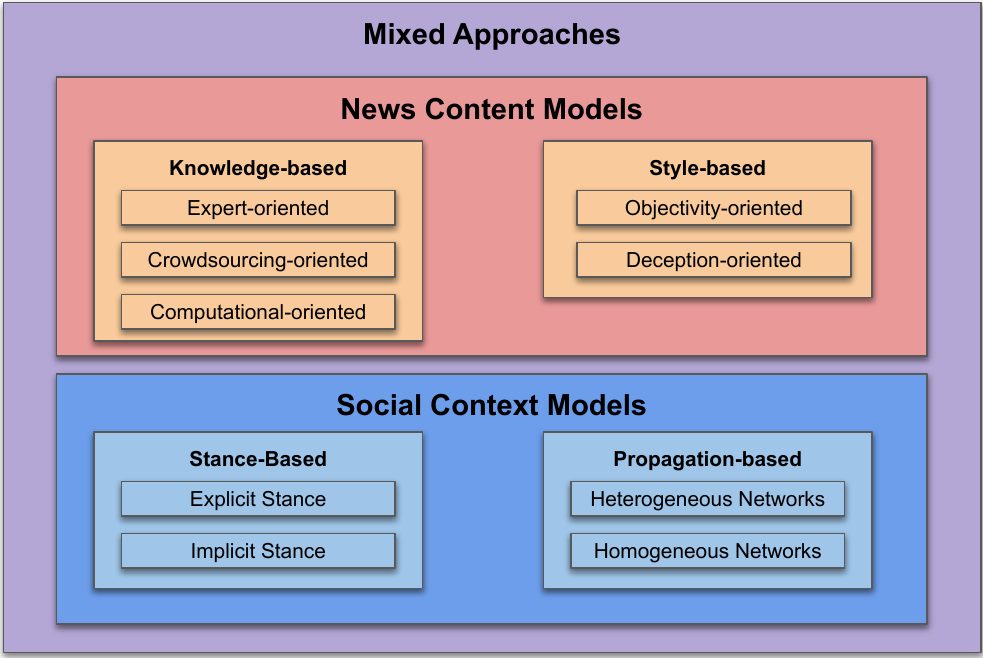
\includegraphics[scale=0.5]{FakeNewsDetectionModelsClassification}
    \caption[Hierarchical Classification of Fake News Detection Models]{Hierarchical Classification of Fake News Detection Models}
    \label{fig:FakeNewsDetectionModelsClassification}
\end{figure}

\textbf{News Content Models.} Based on news content and fact-checking methodologies, these models are the starting point of fake news detection. News content models are classified as Knowledge-based and Style-based. We first introduce style-based models as they are the initial approaches for FND.
\begin{description}
    \item{\emph{Style-based}:} Previous research in psychology has mainly focused on style-based approaches to detect \emph{manipulators} in the text. Particularly deception detection techniques were popular and commonly developed in early works in criminology and psychology. We describe two different ways to approach style-based news content models, namely, \emph{Deception-oriented} and \emph{Objectivity-oriented}~\parencite{FakeNewsDetectionOnSocialMediaADataMiningPerspective_Shu}.
    \begin{itemize}
        \item \emph{Deception-oriented}: The initial approaches for automated fake news detection focus on news context and stem from deception detection in language. The first study that focuses deception detection in language~\parencite{DieEntwicklungDerGerichtspsychologischen_Undeutsch} hypothesized that the truthfulness of the statement is more important than the integrity of the reporting person, and there exist definable and descriptive criteria that form a crucial mechanism for the determination of the truthfulness of statements. Even though this study is from experimental psychology, it stresses the feasibility of defining a set of rules that determine the truthfulness of a statement.\\ An early study from criminology, Scientific Content Analysis (SCAN)~\parencite{SCAN_Sapir1987}, analyzes freely written statements.  In this process, SCAN claims to detect potential instances of deception in the text but cannot label a statement as a lie or truth. The next study for SCAN~\parencite{SCAN_Smith2001} is the first known study that correlates linguistic features with deceptive behavior using high-stakes data. Similar to SCAN, the subsequent studies  ~\parencite{CommunicationUnderStress_Adams, LyingWords_Newman} that link linguistic features to deception classify the owner of the statement as truth-teller or liar according to the frequency of deception indicators in the statement.\\Although for automated deception detection, defining a methodology is more challenging~\parencite{TheAccuracyConfidenceRelation_DePaulo}, early studies have shown that this task is achievable. A detailed study~\parencite{AutomatingLinguisticsBasedCues_Zhou} makes a structured approach using linguistic-based cues and draws attention to further studies for automating deception detection. In this study, the authors extend linguistic-based cues with complexity, expressivity, informality, and content diversity. Instead of using humans as cue identifiers, authors use \emph{Natural Language Processing} (NLP) techniques, namely an NLP tool called iSkim~\parencite{iSkim_Zhou}, to extract cues automatically. Another study also focuses on linguistic cue analysis. With a small dataset and employing the C4.5~\parencite{C45_Salzberg} algorithm, the authors reach 60.72\% accuracy using 15-fold cross-validation.\\Similarly, in ~\parencite{VerificatoinAndImplementationofLBDeceptionIndicators_Bachenko}, the authors developed a system for automatically identifying 275 truthful or deceitful statements with the use of verbal cues using Classification and Regression Tree (CART)~\parencite{ClassificationRegressioniTrees_Breiman}. Additionally, the studies ~\parencite{OnLyingAndBeingLiedTo_Hancock, OnDeceptionAndDeceptionDetection_Rubin} make use of a relatively small dataset and analyze linguistic-based cues. Rubin’s series of  studies~\parencite{OnDeceptionAndDeceptionDetection_Rubin, IdentificationOfTruth_Rubin, TruthAndDeception_Rubin, TowardsNewsVerification_Rubin} makes use of Rhetorical Structure Theory (RST) and Vector Space Modeling (VSM). The first captures the coherence of a story using functional relations among meaningful text units and delivers a hierarchical structure for each news story~\parencite{RST_William}. The second is the way to represent rhetorical relations in high-dimensional space. The authors utilized logistic regression as their classifier and reached 63\% accuracy.\\Furthermore, a study from Afroz and colleagues~\parencite{DetectingHoaxesFraudsAndDeception_Afroz} investigates stylistic deception and uses lexical, syntactic, and content-specific features. Lexical features include both character- and word-based features. Syntactic features represent sentence-level style and include frequency of function words from LIWC~\parencite{LIWC2007_Pennebaker}, punctuation, and POS tagging in which a text is assigned its morphosyntactic category~\parencite{POS_Daelemans}. Finally, content-specific features are keywords for a specific topic. For classification, the authors then leveraged Support Vector Machines (SVM)~\parencite{SVM_Hearst}. More comprehensive and modern approaches such as~\parencite{LiarLiarPantsOnFire_Wang} also leveraged the power of \emph{Convolutional Neural Networks} (CNN) to determine the veracity of news.
        \item \emph{Objectivity-oriented}: Objectivity-oriented news content models aim to detect indicators of the lessening of objectivity in news content~\parencite{FakeNewsDetectionOnSocialMediaADataMiningPerspective_Shu}. These indicators are observed in the news from misleading sources, such as hyperpartisan sources which display highly polarized opinions in favor of or against a particular political party. Consequently, this polarized behavior motivates the fabrication of news that supports the sources’ political views or undermines the opposing political party. \emph{Hyperpartisan news} are a subtle form of fake news and  defined as misleading coverage of events that did actually occur with a strong partisan bias~\parencite{FightingMisinformationOnSocialMedia_Pennycook}. Since the spread of hyperpartisan news can be detrimental, many approaches to detect hyperpartisanship in news articles have been developed. For instance, in~\parencite{AStylometricInquiry_Potthast}, the authors take a stylometric methodology to detect hyperpartisan news. In this study, the authors employ 10 readability scores, and dictionary features where each feature represent the frequency of words from a carefully crafted dictionary in a given document with the help of General Inquirer Dictionaries~\parencite{TheGeneralInquirer_Stone}. A competition for detecting hyperpartisan news~\parencite{SemEvalHyperpartisanNewsDetection_Kiesel} hosted several teams with a variety of ideas which include the utilization of n-grams, word embeddings, stylometry, sentiment analysis etc. The most popular method was the usage of embeddings, particularly the models that leveraged BERT~\parencite{BERT_Devlin}.\\ Also used for dissemination of hyperpartisan news~\parencite{SemEvalHyperpartisanNewsDetection_Kiesel}, another form of fake news that is evaluated under this focus is \emph{Yellow-journalism}, which utilizes clickbaits such as catchy headlines, images etc. that invokes strong emotions, and it aims to generate revenue~\parencite{ClickbaitDetectionUsingDL_Agrawal, ClickbaitAndTabloidStrategies_Dolors}. Studies that aim to detect clickbaits mainly focus on headlines. For example, in~\parencite{DivingDeepIntoClickbaits_Rony}, the authors construct a DNN in which they use distributed subword embeddings~\parencite{EnrichingWordVectorsWithSubwordInfo_Bojanowski, BagOfTricksForTextClassificatoin_Joulin} as features with an extension of skip-gram model~\parencite{DistributedRepresentationsOfWords_Mikolov}.
    \end{itemize}
    \item{\emph{Knowledge-based}}: Being the most direct way for detecting fake news, these approaches make use of external fact-checkers to verify the claims in news content~\parencite{FakeNewsDetectionOnSocialMediaADataMiningPerspective_Shu}. Fact-checkers are either sophisticated algorithms, domain experts or crowdsourced to assess the truthfulness to a claim in a specific context~\parencite{FactChecking_Vlachos}. With growing attention on fake news detection, automated fact-checking has drawn much attention and considerable efforts have been made in this area~\parencite{AutomatedFactChecking_Thorne, OverviewOfCheckThat_Barroncede}. We categorize knowledge-based news content models as \emph{Expert-oriented}, \emph{Crowdsourcing-oriented}, and \emph{Computational-oriented}~\parencite{FakeNewsDetectionOnSocialMediaADataMiningPerspective_Shu}.
    \begin{itemize}
        \item \emph{Expert-oriented}: These approaches are essentially dependent on human domain experts who investigate the integrity of a
              news piece collecting relevant information and documents to come up with a decision about the truthfulness of a
              claim\footnote{https://www.politifact.com/article/2018/feb/12/principles-truth-o-meter-politifacts-methodology-i/}. Platforms
              like Politifact\footnote{https://www.politifact.com/} and EUfactcheck\footnote{https://eufactcheck.eu/} are examples for expert-oriented fact-checking for all news from a variety of sources. These platforms label news in a range such that the label reflect the veracity of news. A different approach for labeling is exercised by Snopes\footnote{https://www.snopes.com/}, which extends the same logic of Politifact by including different aspects of fact-checking such as Scam, Miscaptioned, Outdated
              etc\footnote{https://www.snopes.com/fact-check-ratings/}. Recently replaced by an irrelevant magazine website, another instance was Gossipcop\footnote{https://web.archive.org/web/20190807002653/https://www.gossipcop.com/about/}, which dealt with celebrity fact-checking and contributed to the creation of fake news dataset~\parencite{FakeNewsNet_Shu}. Even though expert-based fact-checking is reliable, with the increasing magnitude of news stream and speed of spreaed, it is not scalable to fact-check every news piece by hand, thus manual validation alone becomes insufficient~\parencite{ASurveyOnAutomatedFactChecking_Guo}.
        \item \emph{Crowdsourcing-oriented}: Powered by wisdom of crowds~\parencite{WisdomOfCrowds_Galton}, crowdsourcing-oriented fact-checking
              is a collection of annotations which are afterwards aggregated to obtain an overall result indicating the veracity of news. Unlike professional fact-checkers, who are in short supply, this approach is scalable given that the crowd contains enough literate people~\parencite{ScalingUpFactChecking_Allen}.  For instance, Twitter launched a program called
              Birdwatch\footnote{https://twitter.github.io/birdwatch/overview/}, in which the users are able to leave notes for tweets that they
              think contains misinformation. Furthermore, this tool allows users to rate each other’s notes, leading to the diversity of perspectives\footnote{https://twitter.github.io/birdwatch/diversity-of-perspectives/}. Another example is from
              Facebook\footnote{https://www.facebook.com/formedia/blog/third-party-fact-checking-how-it-works}, which uses a third party of
              crowdsourced fact-checkers called International Fact-Checking Network\footnote{https://www.poynter.org/ifcn/} (IFCN).
        \item \emph{Computational-oriented}: Heavily dependent on external sources, computational-oriented models are scalable automated
              systems that is designed to predict whether a claim is truthful or not. The studies that focused on this type of approaches mainly try
              to solve two issues: (i) identifying check-worthy claims, and (ii) estimating the integrity of
              claims~\parencite{FakeNewsDetectionOnSocialMediaADataMiningPerspective_Shu}.  The first issue requires extraction of factual claims from news content or other related textual content. For example, in~\parencite{DetectingCheckWorthyClaims_Hassan} the authors collect presidential debate transcripts, then label them into three classes with the help of crowdsourcing. Using annotated data and supervised learning techniques, the authors uncover some interesting patterns in these transcripts. Another study that covers both issues uses wikipedia information to generate factual claims then check whether a given claim is truthful or not~\parencite{FEVER_Thorne}.  The second issue, compared to the first one, requires utilization of structured external sources. \emph{Open web} and structured \emph{knowledge graphs} are two most prominent tools when tackling this issue. Open web tools analyze features like mutual information statistics~\parencite{UnsupervisedNamedEntityExtraction_Etzioni}, frequency, and web-based statistics~\parencite{WebBasedStatisticalFactChecking_Magdy}.  On the other hand, knowledge graphs are interconnected. One noteworthy example is ongologies such as DBPedia~\parencite{DBPedia_Auer}, using which one can define semantic relations and rules in order to infer whether a claim is correct~\parencite{SemanticFakeNewsDetection_Bracsoveanu}.
    \end{itemize}
\end{description}

\textbf{Social Context Models}








\section{Explainable Artificial Intelligence}
\label{sec:explainableArtificialIntelligence}

\subsection{Importance of Explainable Artificial Intelligence}

\subsection{A Good Explanation}

\subsection{Overview of Explainable Artificial Intelligence}
only include what you use.
